\documentclass[a4paper,12pt]{report}
\usepackage[left=2cm,right=2cm,top=2.2cm,bottom=2.2cm]{geometry}
\usepackage{fontspec}
\usepackage{xeCJK}
\usepackage{amsmath}
\usepackage{booktabs}
\usepackage{graphicx}
\usepackage{float}
\usepackage{enumitem}
\graphicspath{{../outputs/}}

\setmainfont{Times New Roman}
\setCJKmainfont{Microsoft JhengHei}
\setlength{\parindent}{0pt}
\setlength{\parskip}{0.45em}
\renewcommand{\tablename}{表}
\renewcommand{\figurename}{圖}

\title{\textbf{SECOM 半導體製程資料 Phase I/II 修正版分析}}
\author{學號：611211106\\統計專論（三）Final Report}
\date{2026 年 6 月 17 日}

\begin{document}
\maketitle
\tableofcontents

\chapter{修正重點}

本次修正依照報告後老師的建議，將分析流程改為先將原始時間序列資料切分為 Phase I 與 Phase II，再只對 Phase I 做資料前處理。Phase I 先刪除缺失值，再使用 3 倍 IQR 規則移除離群值；Phase II 則視為新取得資料，不做離群值刪除。

由於選用變數 \(x_{297}\) 呈現嚴重右偏，後續不再使用以常態假設為基礎的 EWMA、CUSUM 與 CPD 管制界線作為 Phase II 偵測工具。Individuals Shewhart chart 改以 Phase I 配適 Gamma 分配建立上管制界線，下管制界線設為 0。Phase II 的主要診斷則改採整段 Phase II 的無母數 RS/P 診斷。

\chapter{資料切分與前處理}

本分析使用 SECOM 資料中的單一製程變數 \(x_{297}\)。原始資料共 1567 筆，依時間排序後以 \(m=\lfloor n/2 \rfloor\) 切分。

\begin{table}[H]
\centering
\caption{Phase I / Phase II 原始切分}
\begin{tabular}{lrl}
\toprule
階段 & 原始筆數 & 說明 \\
\midrule
Phase I & 783 & 用於建立參考樣本與管制界線 \\
Phase II & 784 & 視為新取得資料，不做離群值刪除 \\
\bottomrule
\end{tabular}
\end{table}

Phase I 前處理結果如下。離群值規則只使用 Phase I 樣本估計，不使用 Phase II 資訊。

\begin{table}[H]
\centering
\caption{Phase I 前處理摘要}
\begin{tabular}{lr}
\toprule
項目 & 數值 \\
\midrule
Phase I 原始筆數 & 783 \\
Phase I 缺失值刪除 & 2 \\
Phase I 3 IQR 離群值刪除 & 24 \\
Phase I 清理後筆數 & 757 \\
3 IQR 下界 & -4376.27 \\
3 IQR 上界 & 7265.77 \\
\bottomrule
\end{tabular}
\end{table}

Phase II 不做離群值刪除。本資料的 Phase II 中 \(x_{297}\) 無缺失值，因此整段 784 筆皆可用於 RS/P 診斷。

\begin{figure}[H]
\centering
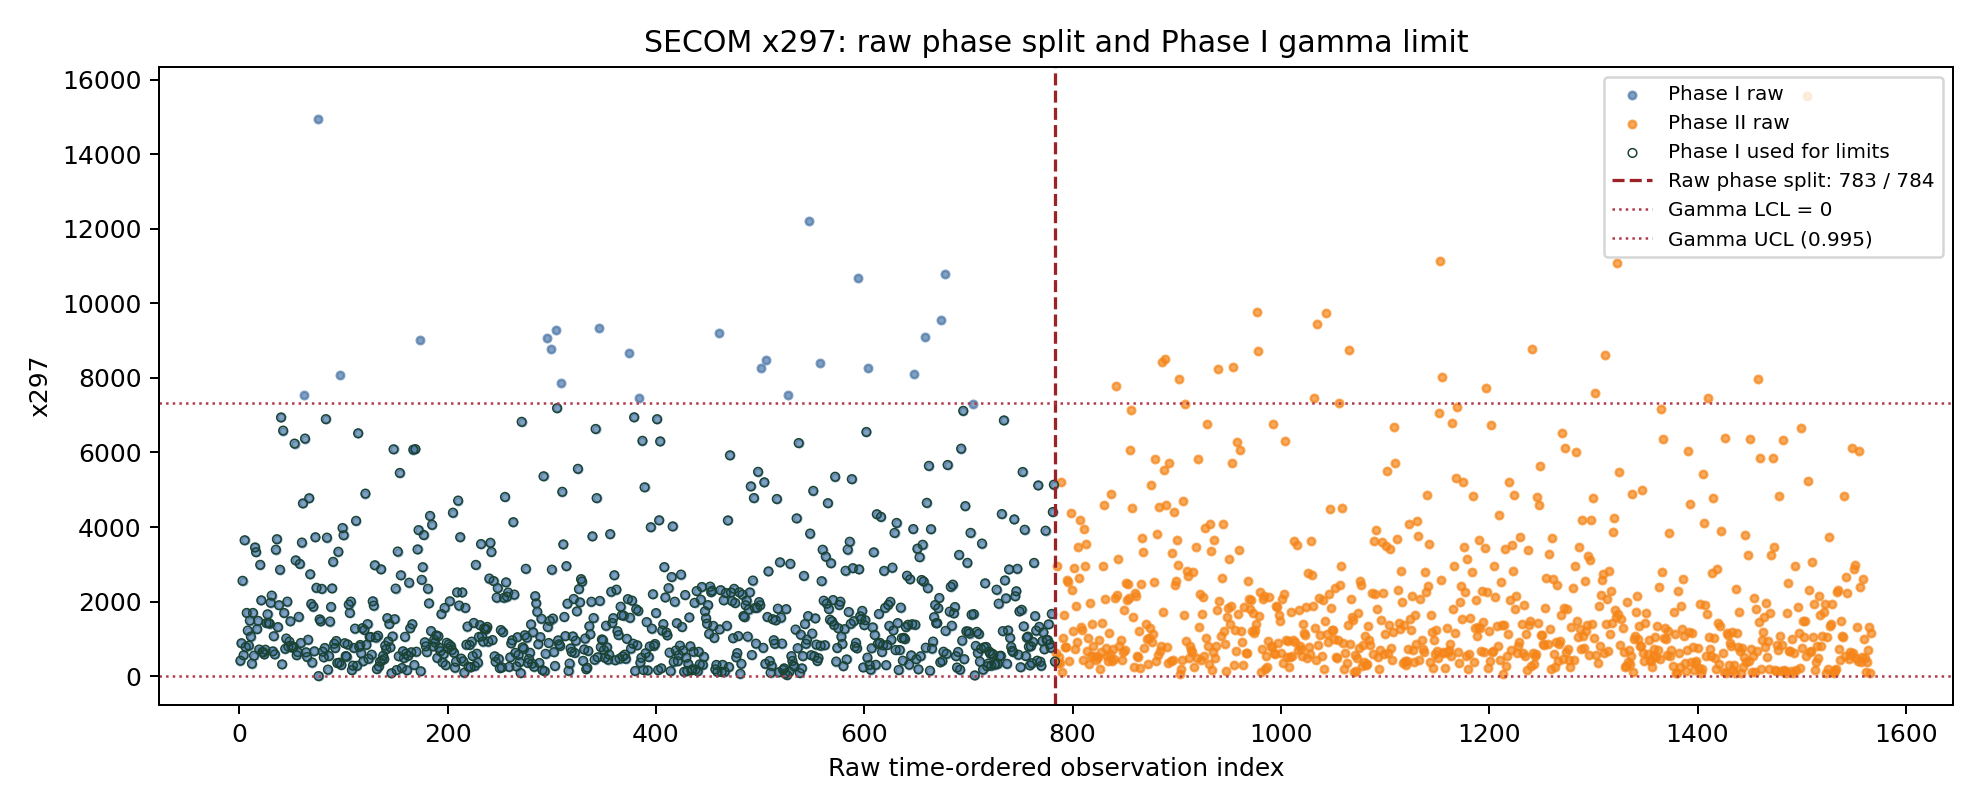
\includegraphics[width=0.95\linewidth]{series_phase_split.png}
\caption{原始資料切分與 Phase I Gamma 管制界線}
\end{figure}

\chapter{Phase I 診斷與 Gamma 管制界線}

清理後 Phase I 的 \(x_{297}\) 摘要如下。平均數大於中位數，最大值也遠高於第三四分位數，顯示資料明顯右偏。

\begin{table}[H]
\centering
\caption{清理後 Phase I 描述統計}
\begin{tabular}{rrrrrrr}
\toprule
平均數 & 標準差 & 最小值 & Q1 & 中位數 & Q3 & 最大值 \\
\midrule
1629.34 & 1478.01 & 0.00 & 598.12 & 1141.48 & 2109.16 & 7189.73 \\
\bottomrule
\end{tabular}
\end{table}

Phase I 用於建立 in-control reference sample，因此仍先以 RS/P 方法檢查清理後 Phase I 是否有明顯 level 或 scale 變化。

\begin{table}[H]
\centering
\caption{Phase I RS/P 穩定性診斷}
\begin{tabular}{lrrr}
\toprule
診斷 & p-value & 最大統計量 & 估計切點 \\
\midrule
Level & 0.9650 & 1.5446 & 82 \\
Scale & 0.7450 & 2.7315 & 34 \\
\bottomrule
\end{tabular}
\end{table}

兩個 p-value 皆大於 0.05，因此沒有足夠證據認為清理後 Phase I 有明顯 level 或 scale 不穩定。Phase I 可作為後續建立管制界線的參考資料。

考量 \(x_{297}\) 為非負且右偏，本次不採用常態 3-sigma limits。Individuals Shewhart chart 改以 Gamma 分配估計上管制界線，下管制界線固定為 0。Gamma 分配配適時，Phase I 中有 1 筆為 0，因此配適 shape 與 scale 時使用正值樣本。

\begin{table}[H]
\centering
\caption{Gamma Individuals Shewhart 管制界線}
\begin{tabular}{lr}
\toprule
參數 & 數值 \\
\midrule
Gamma shape & 1.3607 \\
Gamma scale & 1199.0099 \\
Gamma location & 0 \\
上管制界線 UCL & 7338.8437 \\
下管制界線 LCL & 0 \\
Phase II 超過 UCL 筆數 & 23 \\
Phase II 第一個超過 UCL 的原始 index & 842 \\
\bottomrule
\end{tabular}
\end{table}

\begin{figure}[H]
\centering
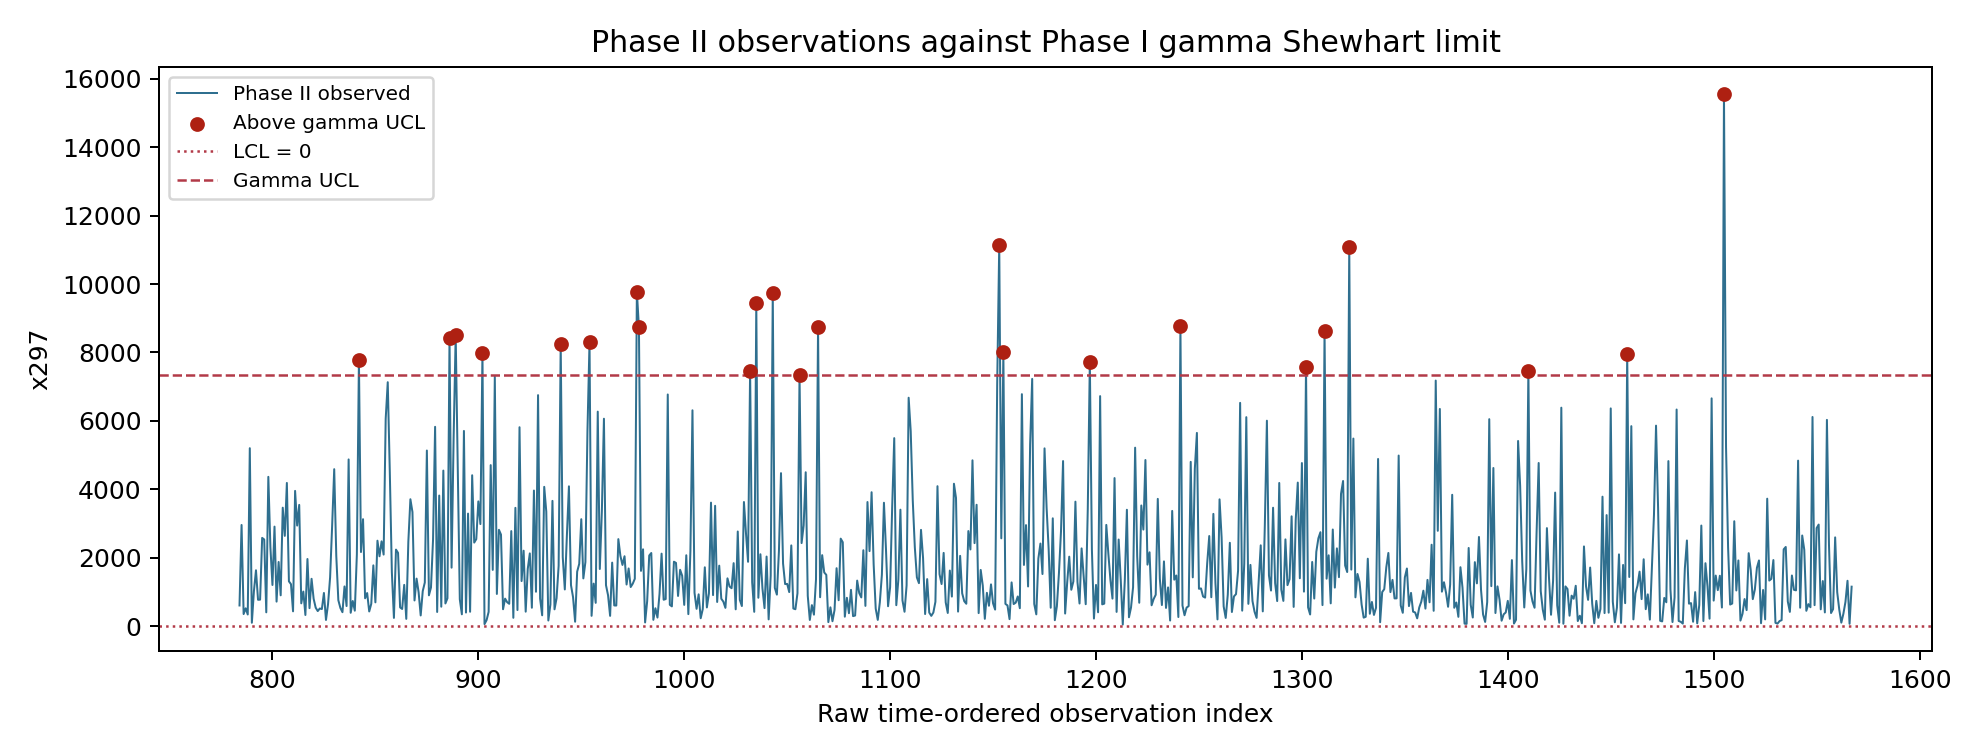
\includegraphics[width=0.95\linewidth]{phaseii_gamma_shewhart.png}
\caption{Phase II 觀測值與 Gamma Shewhart 上管制界線}
\end{figure}

\chapter{Phase II 整段 RS/P 診斷}

Phase II 不做離群值刪除，直接使用整段 784 筆資料進行 RS/P 診斷。

\begin{table}[H]
\centering
\caption{Phase II 整段 RS/P 診斷}
\begin{tabular}{lrrrr}
\toprule
診斷 & p-value & 最大統計量 & Phase II 估計切點 & 原始 index \\
\midrule
Level & 0.0575 & 6.9002 & 776 & 1559 \\
Scale & 0.1000 & 17.5997 & 776 & 1559 \\
\bottomrule
\end{tabular}
\end{table}

在 0.05 顯著水準下，整段 Phase II 的 level 與 scale 診斷皆尚未達顯著。不過 \(p_{\text{level}}=0.0575\) 已接近 0.05，且 level 與 scale 的估計切點都落在 Phase II 後段，對應原始 index 1559。這表示 Phase II 後段可能有需要進一步檢查的結構變化。

\begin{figure}[H]
\centering
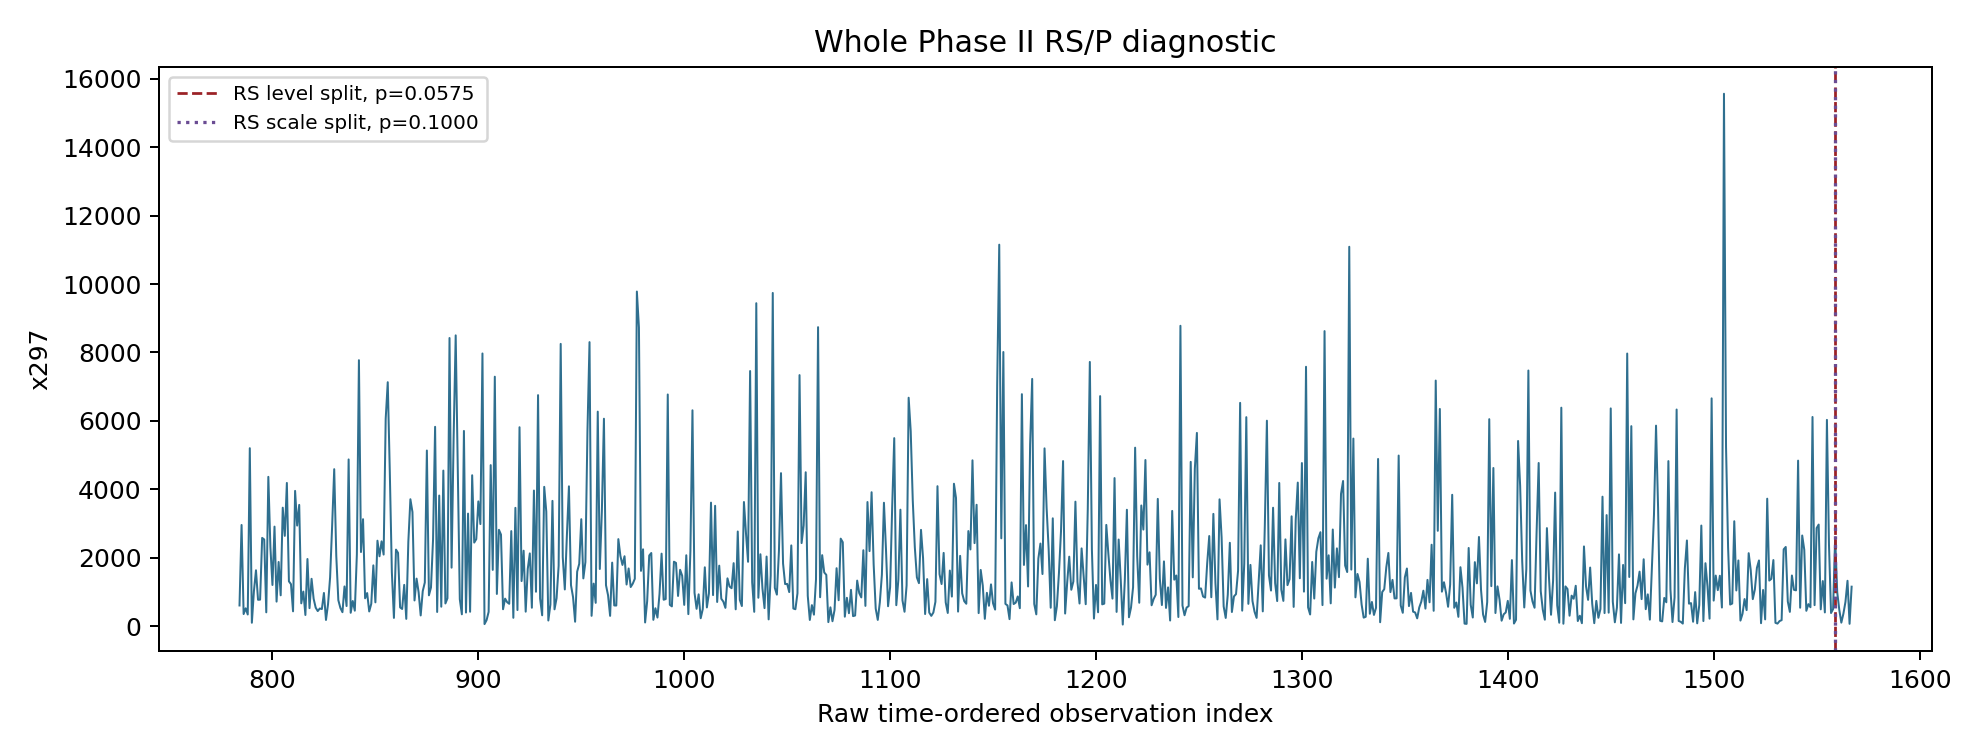
\includegraphics[width=0.95\linewidth]{phaseii_rsp_diagnosis.png}
\caption{整段 Phase II 的 RS/P 診斷位置}
\end{figure}

\chapter{結論}

本次修正後，分析流程更符合 Phase I/Phase II 監控架構。Phase I 清理後可視為穩定參考樣本，並以 Gamma 分配建立非負右偏資料較合理的 Individuals Shewhart 管制界線。Phase II 保持原始狀態，整段 RS/P 診斷在 0.05 水準下尚未顯著，但 level 診斷接近顯著，且估計切點落在 Phase II 後段。

EWMA、CUSUM 與原本使用的 CPD 管制界線主要依賴常態或近似常態下的統計量校準。因 \(x_{297}\) 嚴重右偏且非負，本次不再將這些方法作為 Phase II 管制圖結果呈現。

後續建議是針對 Phase II 進一步做分段 RS/P 診斷，例如以滑動視窗或分批抽樣方式檢查後段是否穩定。若多個區段都顯示後段 level 或 scale p-value 偏小，則可更有根據地指出 Phase II 後段存在製程結構變化。

\end{document}
